%!TEX TS-program = pdflatex
\documentclass[11pt, letterpaper]{article}

\usepackage[english]{babel}
\usepackage{ragged2e}
\usepackage{tabularx}

%% Underline (for URLs)
\usepackage{soul}
\setul{2pt}{0.7pt} % {distance}{thickness}

%% Colors
\usepackage[dvipsnames,svgnames]{xcolor}
\definecolor{jldOrange}{HTML}{f4c472}          % Dandelion
\definecolor{jldOrangeText}{HTML}{EEAE42}      % Slightly darker Dandelion
\definecolor{jldLightOrange}{HTML}{fcf0db}     % Lighter Orange variation
\definecolor{jldHighlight}{HTML}{f5e6cb}       % Highlight Orange variation
\definecolor{jldGray}{HTML}{7b7d80}            % A soft shade of Gray 1
\definecolor{jldGray2}{HTML}{5c5c5c}           % A soft shade of Gray 2
\definecolor{jldWarmBeige}{HTML}{e4d4bf}       % A shade of Beige

%% Highlight for extra emphasis
\usepackage{tikz}
\newcommand{\cvtag}[1]{%
  \tikz[baseline]\node[anchor=base,fill=jldLightOrange,text=black, rounded corners=0.5ex,inner xsep=1ex,inner ysep =0.55ex,text height=1.7ex,text depth=.25ex]{#1};
}

%% Geometry
\usepackage[left=0.65in, right=1in, vmargin=0.75in]{geometry}

%% Font
\usepackage[oldstylenums]{kpfonts}
\usepackage[T1]{fontenc}
\usepackage[final]{microtype}

%% Items
\usepackage{enumitem}
\setlist[itemize]{left=0ex, label=\rule[0ex]{1.3ex}{1.3ex}, labelsep=2ex, font=\color{jldOrange}} % \faCaretRight

%% URLs
\usepackage{xurl}
\usepackage[hidelinks]{hyperref}
\newcommand{\link}[2]{\href{#1}{\setulcolor{jldOrangeText}\ul{#2}}}
\usepackage{bookmark}

%% Figures
\usepackage{graphicx}
\usepackage[absolute,overlay]{textpos}

%% Title formatting
\usepackage{titlesec}
\setlength{\parindent}{0pt}
\titleformat{\section}{\Large\scshape\raggedright}{}{0em}{}

%% No page numbering
\pagenumbering{gobble}


% -----------------------------------------------------------------------------

\newcommand{\name}{Ali Bozorgzadeh}
\newcommand{\whoAmIShort}{CFD \& Scientific Computing Enthusiast}
\newcommand{\bachelorUniversity}{Babol Noshirvani Uni. of Tech.}
\newcommand{\masterUniversity}{Babol Noshirvani Uni. of Tech.}

%------------------------------------------------------------------------------

\begin{document}

%==============================================================================
% "business card" section
%==============================================================================

\begin{minipage}[t][1.25in][t]{.5\textwidth}
\begin{tabular}{@{}l@{}} % @{} removes tabular outer padding
\\
{\Huge\scshape \name}
\begin{textblock*}{\textwidth}(8.4cm,2.2cm) % Width of the block and position (x,y)
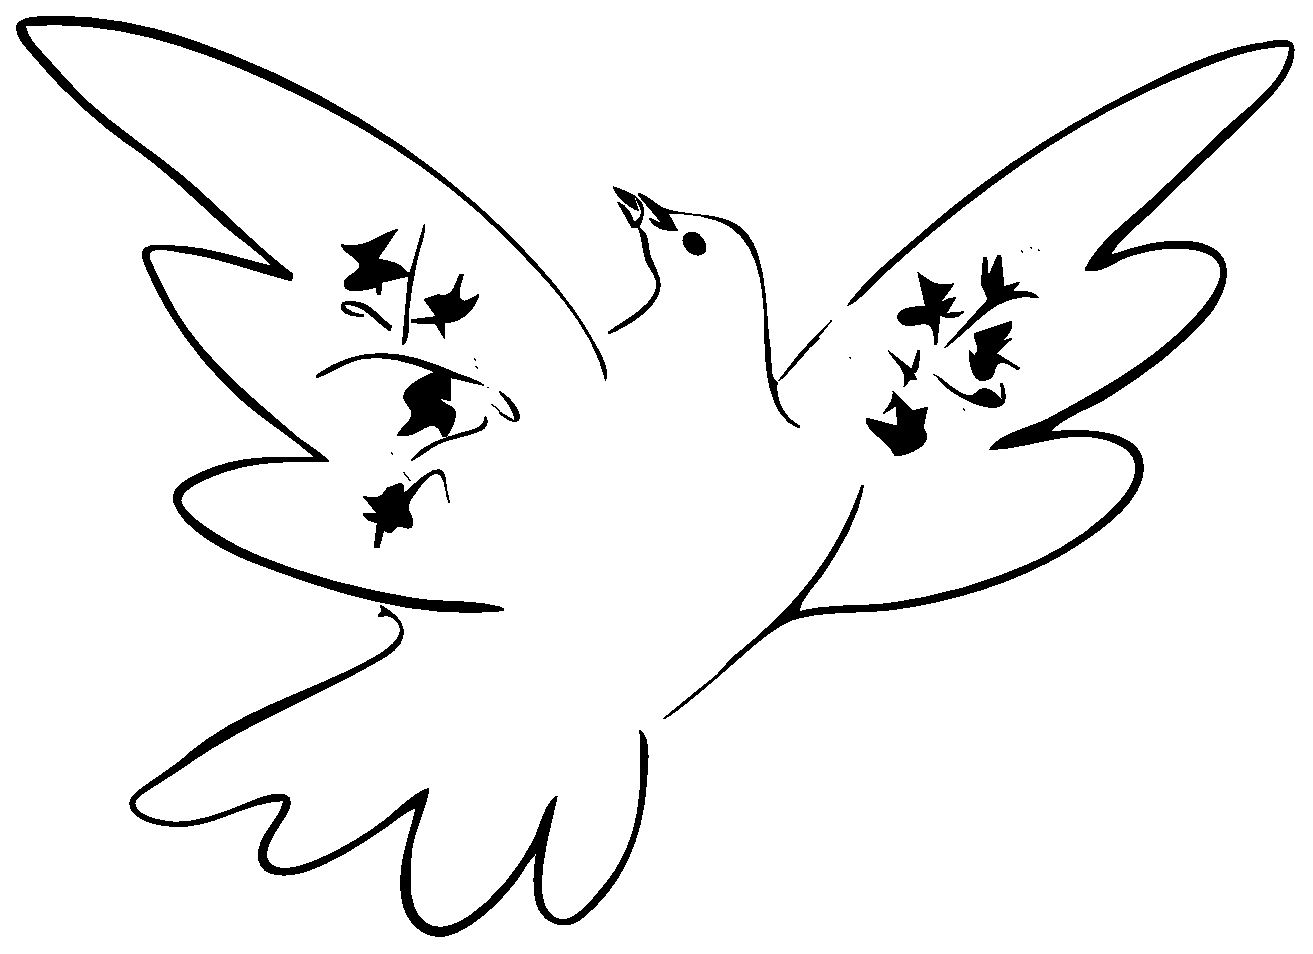
\includegraphics[width=0.35\linewidth]{./figures/Dove.eps}
\end{textblock*}
\\[2.35ex]
{\large\itshape \color{jldGray} \whoAmIShort}
\end{tabular}
\end{minipage}
\hfill
\begin{minipage}[t][1.25in][t]{.3\textwidth}
\hfill
\begin{tabular}{l@{}}
    \href{mailto://alixbozorgzadeh@gmail.com}{\color{jldGray}alixbozorgzadeh\textcolor{jldGray!50}{@gmail.com}} \\
    \href{https://linkedin.com/in/alibozorgzadeh}{\color{jldGray}\textcolor{jldGray!50}{in/}alibozorgzadeh} \\
    \href{https://github.com/abzrg}{\color{jldGray}\textcolor{jldGray!50}{gh/}abzrg} \\
    \href{https://abzrg.github.io}{\color{jldGray}abzrg\textcolor{jldGray!50}{.github.io}}
\end{tabular}
\end{minipage}

\vspace{-2ex}
% \vspace{-2ex}
% My graduate research focused on CFD simulations of various fluid mechanics
% phenomena, including \emph{mass transport in water desalination devices} and
% \emph{particle separation in microfluidic systems}. Currently, my interests lie
% in \emph{Fluid-Solid Interaction} and the application of \emph{neural
% networks} in fluid mechanics.

%==============================================================================
% detail section
%==============================================================================

\section{Education}
\begin{tabularx}{\textwidth}{p{45mm} X}
    \textcolor{jldGray}{2018} -- 2022 & \textbf{M.Sc. in Mechanical Engineering}, \textsc{\color{jldGray}\masterUniversity}
    \\
                                      & \begin{itemize}[noitemsep,nolistsep]
                                          \item {\color{jldGray}Topic:} Investigation of the Effect of Flow Pulsation and Increased Discharged Voltage on Desalination and Energy Usage of Capacitive Deionization. (\link{https://github.com/abzrg/cdiFoam}{code})
                                          \item {\color{jldGray}GPA:} 3.65/4
                                          % \item I implemented a custom OpenFOAM \link{https://github.com/abzrg/cdiFoam}{solver} to simulate salt absorption/desorption in flow-between mode.
                                        \end{itemize}
    \\[0.5ex]
    \textcolor{jldGray}{2013} -- 2018 & \textbf{B.Sc. in Mechanical Engineering}, \textsc{\color{jldGray}\bachelorUniversity}
\end{tabularx}


\vspace{8ex}

\section{Experience}
\renewcommand{\arraystretch}{1.1}
\begin{tabularx}{\textwidth}{p{45mm} X}
    \textcolor{jldGray}{2022} -- 2023 & \textbf{Research Assitant}, \textsc{\color{jldGray}\masterUniversity}
    \\
                                      & \begin{itemize}[noitemsep,nolistsep]
                                           \item \textcolor{jldGray}{Topic:} Particle separation using dielectrophoresis and a gradient in momentum due to a wall-mounted obstacle. (\link{https://www.sciencedirect.com/science/article/abs/pii/S0021967323003059}{paper}; \link{https://github.com/abzrg/dep\_project}{code})
                                           % \item During this project, I developed OpenFOAM \link{https://github.com/abzrg/dep\_project}{code} consisting of a solver for solving fluid flow and electric potential equations, as well as a custom Lagrangian particle force.
                                       \end{itemize}
    \\
    2022                              & \textbf{Teaching Assitant}, \textsc{\color{jldGray}\masterUniversity}
    \\
                                      & I prepared a series of \link{https://www.youtube.com/playlist?list=PLdtuHsHJY9ejxkbkqBSpIHpGfhgte7cbY}{video tutorials} on developing custom OpenFOAM code.
\end{tabularx}
\renewcommand{\arraystretch}{1.0}


\vspace{4ex}

\section{Publications}
\renewcommand{\arraystretch}{1.5}
\begin{tabularx}{\textwidth}{p{45mm} X}
  2023 &
  % \begin{itemize}[noitemsep,nolistsep]
  %     \item
          \textcolor{jldGray}{Reza Derakhshan, \textbf{Ali Bozorgzadeh}, and Abas Ramiar.}
          Numerical Investigation of Ternary Particle Separation in a Microchannel with a Wall-Mounted Obstacle Using Dielectrophoresis.
          \textcolor{jldGray}{\emph{Journal of Chromatography A} (2023) \textsc{doi}: \link{https://doi.org/10.1016/j.chroma.2023.464079}{10.1016/j.chroma.2023.464079}}
  % \end{itemize} \\
  \\
  2020 &
  % \begin{itemize}[noitemsep,nolistsep]
      % \item
          \textcolor{jldGray}{Masoud Outokesh, Seyed S. M. Ajarostaghi, \textbf{Ali Bozorgzadeh}, and Kurosh Sedighi.}
          Numerical evaluation of the effect of utilizing twisted tape with curved profile as a turbulator on heat transfer enhancement in a pipe.
          \textcolor{jldGray}{\emph{Journal of Thermal Analysis and Calorimetry} (2020) \textsc{doi}: \link{https://link.springer.com/article/10.1007/s10973-020-09336-0}{10.1007/s10973-020-09336-0}}
  % \end{itemize}
\end{tabularx}
\renewcommand{\arraystretch}{1.0}



\section{Personal Projects \& Open-Source Contributions}
\renewcommand{\arraystretch}{1.3}
\begin{tabularx}{\textwidth}{p{45mm} X}
% \link{https://github.com/abzrg/dep\_project}{dep\_project} & Source code of the dielectrophoresis particle separation project (OpenFOAM v2206). \link{https://www.sciencedirect.com/science/article/abs/pii/S0021967323003059}{paper} \\
\link{https://github.com/abzrg/nmpy}{nmpy} & A Python package for simple numerical method algorithms \\
% \link{https://github.com/abzrg/machine\_learning}{machine\_learning} & Collection of ML projects with regression, classification, and PyTorch MLP implementations \\
\link{https://github.com/abzrg/parallel-programming}{parallel-programming} & Parallel programming using Unix processes, Pthreads and OpenMP \\
\link{https://github.com/abzrg/ds}{ds} & Implementation of the Binary Search Tree data structure in C \\
% \link{https://github.com/abzrg/oxpr}{oxpr} & A shell script that downloads (UK/US) pronunciations of a given word \\
Bug-Report \& Docs & solids4foam, OpenFOAM, preCICE (adaptors)
\end{tabularx}
\renewcommand{\arraystretch}{1.0}



\section{Skills}
\renewcommand{\arraystretch}{1.3}
\begin{tabularx}{\textwidth}{p{45mm} X}
  Programming &
  \begin{itemize}
      \item \cvtag{C/C++} OpenFOAM, OpenMP, MPI, Pthreads, OpenGL
      \item \cvtag{Python} Numpy, Matplotlib, Pandas, Scikit-Learn, SymPy
      \item Other programming languages: \textcolor{jldGray!50}{POSIX} Shell, \LaTeX, Lua, Fortran, \textcolor{jldGray!50}{E}Lisp, Javascript, HTML, CSS
  \end{itemize}
  \\
  Tools & Linux, Git, Docker, SSH
  \\
  Other Softwares & Paraview, Inkscape, Blender, Gnuplot, FreeCAD
\end{tabularx}
\renewcommand{\arraystretch}{1.0}



\section{Languages}
\begin{tabularx}{\textwidth}{p{45mm} X}
    English & IELTS 7.0/9.0 (\cvtag{L}7.5, \cvtag{R}8.0, \cvtag{W}6.0, \cvtag{S}7.0) \\
    Persian & Native language
\end{tabularx}



\section{Certificates}
\begin{tabularx}{\textwidth}{p{45mm} X}
    \link{https://www.coursera.org/account/accomplishments/specialization/K0PDJBRMGHCV}{ML Specialization} &
    \begin{itemize}
        \item Supervised Machine Learning: Regression and Classification, \link{https://www.coursera.org/account/accomplishments/records/6IM8DUNQOS9M}{Cert.}
        \item Advanced Learning Algorithms, \link{https://www.coursera.org/account/accomplishments/records/H532N5F8UGYA}{Cert.}
        \item Unsupervised Learning, Recommenders, Reinforcement Learning, \link{https://www.coursera.org/account/accomplishments/records/6IM8DUNQOS9M}{Cert.}
    \end{itemize}
\end{tabularx}



\vspace{-10pt}
\section{References}
\begin{tabularx}{\textwidth}{p{45mm} p{60mm} r}
    Abas Ramiar & Supervisor/Co-author & \link{https://scholar.google.com/citations?user=ew-WXvQAAAAJ\&hl=en}{Google Scholar}  \\
    Kurosh Sedighi & Course instructor/Co-author & \link{https://scholar.google.com/citations?user=RlAAZdwAAAAJ\&hl=en}{Google Scholar} \\
    Mohsen Sheikholeslami & Course instructor/Thesis referee & \link{https://scholar.google.com/citations?user=5cJ2aF0AAAAJ\&hl=en}{Google Scholar}
\end{tabularx}

\end{document}
